\chapter{Artificial Neural Networks}\label{chp:3}

We saw in section \ref{limitations}, that the practical applicability of linear models with fixed basis functions is limited. One alternative is choosing a fixed number of \textcolor{blue}{\emph{adaptive basis functions}}. Here, basis functions are parametrized in a suitable way, and the parameters are adapted during the training in such a way such that the model explains (or “tuned” to) the given data. This approach can be carried out via using \textcolor{blue}{\emph{artificial neural networks}}, which we define in what follows.

\section{Fundamental Aspects}

\begin{definition}[Artificial Neural Network]
For a fixed $L \in \mathbb{N}$, let $n_0, \dots, n_L \in \mathbb{N}, W^{[\ell]} \in \mathbb{R}^{n_{\ell} \times n_{\ell -1}},$ and $b^{[\ell]} \in \mathbb{R}^{n_{\ell}}$ for all $\ell = 1, \dots, L$. Furthermore, let $g^{[\ell]}: \mathbb{R}^{n_{\ell}} \rightarrow \mathbb{R}^{n_{\ell}}$ for $\ell = 1, \dots, L$ be some functions. Then the function $f_{\theta} : \mathbb{R}^{n_0} \rightarrow \mathbb{R}^{n_L}$, which maps an \textcolor{blue}{\emph{input vector}} $x \in \mathbb{R}^{n_0}$ to
\begin{align}
    &f_{\theta}(x) := a^{[L]}, \quad \text{where}\\
    &a^{[0]} := x,\\
    &z^{[\ell]} := W^{[\ell]} a^{[\ell-1]} + b^{[\ell]},\\
    &a^{[\ell]} := g^{[\ell]}(z^{[\ell]}), \Biggr\} \quad \ell = 1, \ldots, L
    \label{eqn:29}
\end{align}

is called an \textcolor{blue}{\emph{artificial neural network}} with \textcolor{blue}{\emph{parameters}} $\theta = (W^{[1]}, b^{[1]}, \ldots, W^{[L]}, b^{[L]})$ and \textcolor{blue}{\emph{activation functions}} $g^{[1]}, \ldots, g^{[L]}$. The matrices $W^{[1]}, \ldots, W^{[L]}$ are called \textcolor{blue}{\emph{weight matrices}}, and the vectors $b^{[1]}, \ldots, b^{[L]}$ are called \textcolor{blue}{\emph{bias vectors}} of $f$.\\

For fixed $x \in \mathbb{R}^n_0$ and $\ell \in \{1, \ldots, L\}$, we call $z^{[\ell]} \in \mathbb{R}^{n_{\ell}}$ \textcolor{blue}{\emph{(net) input vector)}} and $a^{[\ell]} \in \mathbb{R}^{n_{\ell}}$ the \textcolor{blue}{\emph{activation vector)}} in the $\ell$-th layer, where $n_{\ell}$ is the \textcolor{blue}{\emph{width)}} of the $\ell$-th layer. Finally, $f_{\theta}(x)=a^{[L]}$ is the \textcolor{blue}{\emph{output vector)}}, and $L$ is called the \textcolor{blue}{\emph{depth)}} of $f_{\theta}$.
\end{definition}

\begin{figure}[h!]
    \centering
    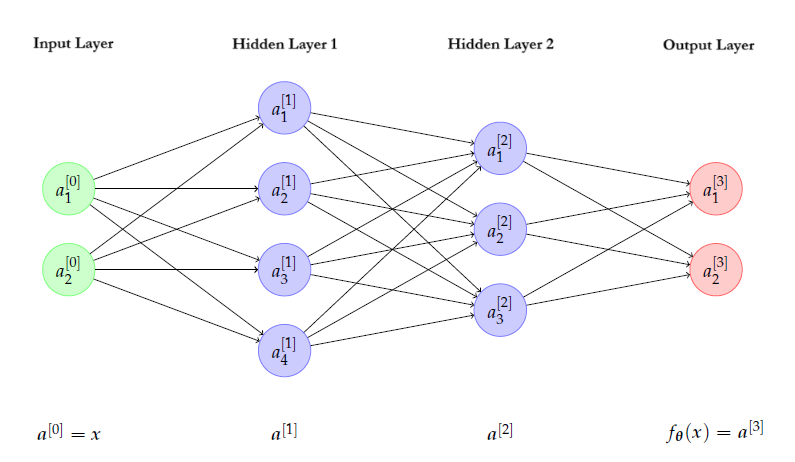
\includegraphics[width=\textwidth]{images/figure6.png}
    \caption{Example of an artificial neural network with two hidden layers.}
    \label{fig:6}
\end{figure}

\begin{remark}[Nonlinearity]
The vectors $a^{[0]}, \ldots, a^{[L]}$ and $z^{[1]}, \ldots, z^{[L]}$ defined in \ref{eqn:29} are, like $f_{\theta}$, functions of the input vector $x$. For simplicity, we usually omit this dependency in our notation as long as the context is clear. Nevertheless, we can understand $f_{\theta}$ as a composition of several linear and nonlinear functions. For example, for $L=1$ we have

\begin{equation}
    f_{\theta}(x) = g^{[1]}(W^{[1]}x + b^{[1]}),
    \label{eqn:30}
\end{equation}\\

meaning that $f_{\theta}$ is a composition of $g^{[1]}$ with $z^{[1]} = W^{[1]}x + b^{[1]}$. Also for $L=2$ we obtain a function

\begin{equation}
    f_{\theta}(x) = g^{[2]}(W^{[2]}(g^{[1]}(W^{[1]}x + b^{[1]})) + b^{[2]}),
    \label{eqn:31}
\end{equation}\\
and the process continues in the same way for $L \geq 3$.\\

In general at least some of the functions $g^{[\ell]}$ are chosen to be nonlinear. If this was not the case, then $f_{\theta}$, as a composition of linear functions, would also be linear. The additional and more complex structure \ref{eqn:29} would therefore have no advantage over a simple representation of the form $f_{\theta}(x) = Wx + b$ with $W \in \mathbb{R}^{n_L \times n_0}$ and $b \in \mathbb{R}^{n_L}$ (as every affine-linear function can be represented in such a way).

\end{remark}

\begin{remark}[Scalar Activation Functions]
The activation function $g^{[\ell]}: \mathbb{R}^{n_{\ell}} \rightarrow \mathbb{R}^{n_{\ell}}$ can often be interpreted as a component-wise application of a real function from $\mathbb{R}$ to $\mathbb{R}$. In this case, unless stated differently, for a scalar function $g^{[\ell]}: \mathbb{R} \rightarrow \mathbb{R}$, we define $g^{[\ell]}(z) \in \mathbb{R}^{n_{\ell}}$ as a component-wise application of $g^{[\ell]}$ to $z \in \mathbb{R}^{n_{\ell}}$,

\begin{equation}
    g^{[\ell]}(z) := \begin{pmatrix}
    g^{[\ell]}(z_1) \\
    \vdots \\
    g^{[\ell]}(z_{n_\ell})
    \end{pmatrix}.
    \label{eqn:32}
\end{equation}

\end{remark}

When defining a neural network, we decide on the type of activation functions that we use.
Below we give a few example of commonly used activation functions.

\begin{example}[Typical Activation Functions]
Depending on the context and goal of the problem, we can use any of the below activation functions (see Figure \ref{fig:7}) while defining the neural network:

\begin{figure}[h!]
    \centering
    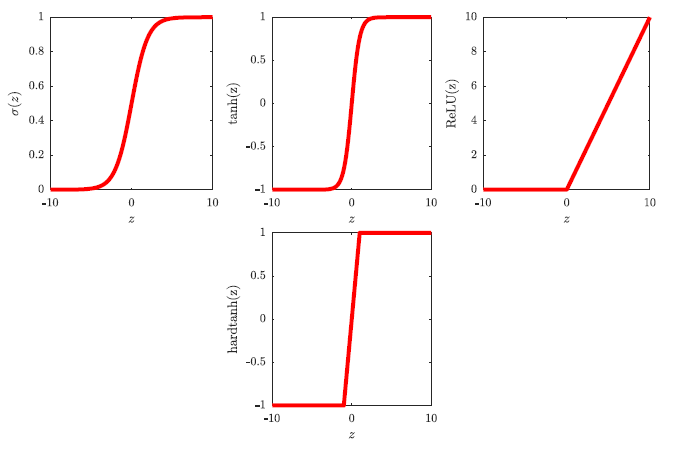
\includegraphics[width=0.8\textwidth]{images/figure7.png}
    \caption{Typical Activation Functions}
    \label{fig:7}
\end{figure}

\begin{itemize}
    \item \textcolor{blue}{\emph{Sigmoid function}}: Commonly used in the output layer of a binary classification task, as it maps values to the range $(0, 1)$, representing probabilities. Suitable when the model needs to output probabilities or interpret values as likelihoods, but it can suffer from vanishing gradients.\cite{hochreiter1997lstm, rumelhart1986learning}
    \begin{equation}
        \sigma: \mathbb{R} \to (0,1), \quad \sigma(z) := \frac{1}{1+e^{-z}}
        \label{eqn:33}
    \end{equation}
    
    \item \textcolor{blue}{\emph{ReLU (Rectified Linear Unit) function}}: It ensures sparsity by retaining only positive activations, which not only introduces non-linearity but also improves computational efficiency and helps avoid the vanishing gradient problem.\cite{nair2010relu}
    \begin{equation}
        \text{ReLU}(z): \mathbb{R} \to \mathbb{R}_{\geq 0}, \quad \text{ReLU}(z) := \max(0, z)
        \label{eqn:34}
    \end{equation}
    
    \item \textcolor{blue}{\emph{Hyperbolic Tangent (tanh) function}}: Preferred in hidden layers when inputs are zero-centered, as it maps the input in the range $(-1, 1)$, which helps faster convergence during training. It has more efficient gradient flow than sigmoid function.
    \begin{equation}
        \text{tanh}: \mathbb{R} \to (-1,1), \quad \text{tanh}(z) := \frac{e^z-e^{-z}}{e^z+e^{-z}}
        \label{eqn:35}
    \end{equation}
    
    \item \textcolor{blue}{\emph{Hard hyperbolic tangent (hardtanh) function}}: Provides a faster approximation of the traditional tanh function, maintaining a balance between non-linearity and computational simplicity.
    \begin{equation}
        \text{hardtanh}(z): \mathbb{R} \to [-1,1], \quad \text{hardtanh}(z) := \max(-1, \min(1,z))
        \label{eqn:36}
    \end{equation}
    
    \item \textcolor{blue}{\emph{Identity function}}: While it does not introduce non-linearity, it is occasionally used in skip connections or output layers when no transformation is needed.
    \begin{equation}
        \text{id}(z): \mathbb{R} \to \mathbb{R}, \quad \text{id}(z) := z
        \label{eqn:37}
    \end{equation}
    
    \item \textcolor{blue}{\emph{Softmax function}}: Typically applied at the output layer for multi-class classification tasks, converting raw scores into normalized probabilities (sums upto $1$). Output values represents a probability distribution over different classes, which is useful when model needs to probability of each class.
    \begin{equation}
        \text{softmax}(z) : \mathbb{R}^n \to \mathbb{R}^n, \quad \text{softmax}(z)_j := \frac{e^{z_j}}{\sum_{j=1}^n e^{z_j}}
        \label{eqn:38}
    \end{equation}
\end{itemize}

\end{example}

\section{Multiclass Classification}
Assume that, in contrast to binary classification, we have not only two but $K$ different classes that we want to assign to elements $x \in \mathcal{X}$ of the sample space. Thus, we have the set $\{0, \ldots, K-1\}$ of $K$ different labels and we seek a \textcolor{blue}{\emph{hypothesis}} of the form $h_{\theta}: \mathbb{R}^d \rightarrow \{0, \ldots, K-1\}$. We realize this approach via the \textcolor{blue}{\emph{One-Hot encoding}}
\begin{equation}
    \{0, \ldots, K-1\} \rightarrow \mathbb{R}^K, \quad k \mapsto e_{k+1}
    \label{eqn:39}
\end{equation}

where $e_{k+1}$ denotes the $(k+1)$-st unit vector, i.e., a vector with $k$ elements, where $k$-th element is $1$, representing $y^{(i)}$ belonging to class $k$. We map every label $y^{(i)} \in \{0, \ldots, K-1\}$ of an element of the training dataset to the corresponding unit vector:

\begin{equation}
    y^{(i)} = e_{y^{(i)}+1} = \begin{pmatrix} 0 \\ \vdots \\ 0 \\ 1 \\ 0 \\ \vdots \\ 0 \end{pmatrix} \leftarrow \text{position } y^{(i)}+1 \in \mathbb{R}^K.
    \label{eqn:40}
\end{equation}

We then use the training data ${(x^{(1)}, y^{(1)}), \ldots, (x^{(m)}, y^{(m)})} \subseteq \mathcal{X} \times \{0, 1\}^K \subseteq \mathbb{R}^d \times \{0, 1\}^K$ and a neural network with input dimension $n_0 =d$ and output dimension $n_L = K$. Further, we determine the depth $L$, widths $n_1, \ldots, n_{L-1}$ of each layer, suitable activation functions $g^{[1]}, \ldots, g^{[L-1]}$ and choose $g^{[L]}:= \text{softmax}$ to be \ref{eqn:38}.

\begin{definition}[Softmax Loss]
The function
\begin{equation}
    \ell : \mathbb{R}^K \times \mathbb{R}^K_{>0} \rightarrow \mathbb{R}, \quad \ell(y, \hat{y}):= -\sum_{k=1}^{K}y_k \ln(\hat{y}_k)
    \label{eqn:41}
\end{equation}
is called \textcolor{blue}{\emph{softmax loss function}}.
\end{definition}

Softmax loss function is often called \textcolor{blue}{\emph{cross-entropy loss function with softmax}} and is a combination of softmax function and cross-entropy loss function. Here, softmax function turns a vector of real-valued scores (often called logits) into a probability distribution over $k$ classes, and the cross-entropy loss function measures how well the predicted probability distribution matches the true distribution. \emph{It is used to quantify the difference between the predicted probability distribution and the actual distribution of class labels in training data}.\\

Let us understand the concept step-by-step:\\

\textbf{Multi-class setting}\\

Let us assume $m$ training samples and $K$ classes. For each training sample $i$, model outputs a logit $z_k^{(i)}$ for each class $k$. These logits are un-normalized real numbers (can be positive or negative), and we want them as a valid probability distribution.\\

\textbf{Softmax function}\\

Softmax of the logits $z_1^{(i)}, z_2^{(i)}, \ldots, z_k^{(i)}$ is defined as:
\begin{equation}
    \hat{y}_k^{(i)} = \text{softmax}(z_k^{(i)}) = \frac{e^{z_k^{(i)}}}{\sum_{j=1}^{K} z_j^{(i)}}
    \label{eqn:42}
\end{equation}
where, $\hat{y}_k^{(i)}$ is the predicted probability that example $i$ belongs to class $k$ and each $\hat{y}_k^{(i)}$ lies in the range $(0,1)$ and the probabilities sum to $1$ across all classes.\\

\textbf{Cross-entropy loss function}\\

To measure how well the predicted probability $\hat{y}_k^{(i)}$ matches the true class, we introduce cross-entropy loss. In a one-hot labeling scheme, each training example $i$ has a label $y^{(i)}$ which is a vector of length $K$ with
\begin{equation}
    y_k^{(i)} =
    \begin{cases}
        1, \quad \text{if example $i$ belongs to class $K$}\\
        0, \quad \text{otherwise}
    \end{cases}
    \label{eqn:43}
\end{equation}

And the cross-entropy loss for example $i$ is:
\begin{equation}
    L^{(i)} = - \sum_{k=1}^{K} y_k^{(i)} \ln (\hat{y}_k^{(i)})
    \label{eqn:44}
\end{equation}
Since, $y_k^{(i)}$ is $1$ for the true class and $0$ otherwise, only the term for the correct class contributes to the sum.\\

\textbf{Combining softmax with cross-entropy}\\

Using the softmax loss function, we will train an artificial neural network $f_{\theta}: \mathbb{R}^{n_0} \rightarrow \mathbb{R}^{n_L}$ by applying an optimization algorithm to the problem:
\begin{equation}
    \min_{\theta \in \Theta} \mathcal{L}(\theta) = \min_{\theta \in \Theta} - \frac{1}{m} \sum_{i=1}^{m} \sum_{k=1}^{K} y^{(i)}_k \ln(\hat{y}_k^{(i)}),
    \label{eqn:45}
\end{equation}

where $\boldsymbol{\theta} = (\boldsymbol{W}^{(1)}, \boldsymbol{b}^{(1)}, \ldots, \boldsymbol{W}^{(L)}, \boldsymbol{b}^{(L)})$ ranges in the set $\Theta$ of parameters of the underlying artificial neural network.\\

Here, our goal is to \textcolor{blue}{\emph{minimize}} the loss function so that the predicted distribution $\hat{y}_k$ is closer to the true distribution $y_k$ as much as possible.\\

\emph{The softmax loss function penalizes the strongly for large errors (low probability assigned to the correct class), hence forcing the model to predict and and correctly assign higher probability to the true class.}\\


To identify the output of $f_{\theta}$ for the $i$-th training sample, we write $\hat{y}^{(i)}:= f_{\theta}(x^{(i)})$ in \ref{eqn:45}. For an object $x$ with unknown label and output $\hat{y} = f_{\theta}(x)$ we then assign the class
\begin{equation}
    h_{\theta}(x) = \left[ \argmax_{k=1, \ldots, K}\text{ } \hat{y}_k \right] - 1
    \label{eqn:46}
\end{equation}

The softmax function defined in \ref{eqn:38} represents a probability distribution over a discrete set. This makes it particularly suitable for the role of the output activation function $g^{[L]}$ for multiclass
classification. For a fixed input vector $x \in \mathbb{R}^d$ and the associated input vector $z^{[L]}$ of the $L$-th layer (output layer), we interpret
\begin{equation}
    \hat{y}_k = \text{softmax}(z^{[L]})_k = \mathcal{D}_{\text{Mod}}(y = k - 1 \mid \boldsymbol{x}; \boldsymbol{\theta}),
    \label{eqn:47}
\end{equation}

which explains why we choose the class with the highest probability in \ref{eqn:46}.\\

For $L=1$ and $z^{[1]} = (-(w^\top x + b),0)$, we obtain

\begin{equation}
\hat{y} = \text{softmax}(z^{[L]}) = \left(\underbrace{1 - \sigma(w^\top x + b)}_{\mathbb{P}(y=0)}, \underbrace{\sigma(w^\top x + b)}_{\mathbb{P}(y=1)}\right)
\label{eqn:48}
\end{equation}

and we see that the Bernoulli distribution \ref{eqn:3} arises as a particular case of \ref{eqn:47}. In particular, logistic regression \ref{eqn:7} is a very special instance of the multiclass classification (with $L = 1$ and \ref{eqn:38} as an output activation function) given by \ref{eqn:46}.\\

In other words, logistic regression is the $2$-class (binary) special case of the general multi-class softmax classification framework. By choosing the logits for class $0$ and class $1$ as $(-(w^\top x + b), 0)$, the softmax probabilities match the Bernoulli distribution used in logistic regression.

\begin{remark}[Maximum Likelihood Interpretation]
As for the cross entropy loss for binary classification, the softmax loss for multiclass classification can be derived via a maximum likelihood approach, where the statistical model is the family of distributions on $\mathcal{X} \times \{0, 1\}^K \subseteq \mathbb{R}^d \times \{0, 1\}^K$ given by \ref{eqn:47}. Using the vector $y \in \{e_1, \ldots, e_K\} \subseteq \mathbb{R}^K$, which is a one-hot encoded label $y \in \{0, \ldots, K-1\}$, we write \ref{eqn:47} as
\begin{equation}
    \mathcal{D}_{\text{Mod}}(y|x;\boldsymbol{\theta}) := \prod_{k=1}^{K} [f_{\theta}(x)_{k}]^{y_k}
    \label{eqn:49}
\end{equation}
Then
\begin{equation}
    \mathcal{L}(\boldsymbol{\theta}) = -\ln \mathcal{D}_{\text{Mod}}(\mathcal{S} ; \boldsymbol{\theta}) = -\ln \prod_{i=1}^{m} \prod_{k=1}^{K} \left[ f_\theta(x^{(i)})_k \right]^{y_k^{(i)}} = - \sum_{i=1}^{m} \sum_{k=1}^{K} y_k^{(i)} \ln f_\theta(x^{(i)})_k
    \label{eqn:50}
\end{equation}
is a negative log likelihood function, where the inner sum corresponds exactly to $\ell(y^{(i)}, f_{\theta}(x^{(i)}))$ from \ref{eqn:41}.
\end{remark}
Let us understand this in detail in the next section.

\section{Maximum Likelihood Estimation}
\emph{Maximum Likelihood Estimation (MLE) is a method used to estimate the parameters of a statistical model that maximizes the likelihood of observing the given data.}

\subsection{Setting up the model}
In a multi-class classification setting with $K$ classes, the goal is to predict the probability of each class given an input $x$. The model outputs a vector of probabilities, $f_{\theta}(x) = (f_{\theta}(x)_1, f_{\theta}(x)_2, \ldots, f_{\theta}(x)_K)$, where each component $f_{\theta}(x)_k$ is the predicted probability that the input $x$ belongs to class $k$.\\

The softmax function (\ref{eqn:38}) is typically used to convert the raw scores (logits) into probabilities, with $z_k$ as the logit (raw score) for class $k$, and $\theta$ represents the parameters of the model.\\

The probability vector $f_{\theta}(x)$ thus satisfies $f_{\theta}(x)_k \in [0,1]$ and $\sum_{k=1}^{K} f_{\theta}(x)_k = 1$.

\subsection{One-Hot encoding of the labels}
For each training example $x^{(i)}$, we assume the true label is $y^{(i)}$, which is a one-hot encoded vector. For instance: $y^{(i)} = (y_1^{(i)}, y_2^{(i)}, \ldots, y_K^{(i)}), \quad y_k^{(i)} \in \{0,1\}, \quad \sum_{k=1}^{K} y_k^{(i)}=1$. For example, if the true class is class $3$, then $y = (0, 0, 1, 0, \ldots, 0)$.\\

Thus, in a multi-class classification problem, the label $y^{(i)}$ is a vector of length $K$, with exactly one element set to $1$ (for the correct class) and all other elements set to $0$.

\subsection{Model distribution}
The statistical model for multi-class classification is based on a family of distributions over the input space $\mathbb{R}^d$ (e.g., feature vectors) and the output space $\{0, 1\}^K$ (e.g., one-hot encoded labels for $K$ classes).

Given the true label $y^{(i)}$ and the predicted probabilities $f_{\theta}(x^{(i)})$, the model is described as below, which is also the probability of correctly predicting the label:
\begin{equation}
    \mathcal{D}_{\text{Mod}}(y^{(i)} \mid x^{(i)}; \boldsymbol{\theta}) = \mathbb{P}(y^{(i)} \mid x^{(i)}; \boldsymbol{\theta}) = \prod_{k=1}^{K}[f_{\theta}(x^{(i)})_k]^{y_k^{(i)}}
    \label{eqn:51}
\end{equation}
where, $y_k$ is the $k$-th component of the one-hot encoded label $y$ and $f_{\theta}(x)$ is the output of the model for input $x$, giving a vector of class probabilities.\\

The equation means that if the true class $y_k^{(i)} = 1$, then we are interested in $[f_{\theta}(x^{(i)})]_k$, the predicted probability for the correct class $k$, but if the true class $y_k^{(i)} = 0$, then that term contributes nothing to the product (because any number raised to the power $0$ is $1$).\\

Thus the above expression in (\ref{eqn:51}) simplifies to:
\begin{equation}
    \mathbb{P}(y^{(i)} \mid x^{(i)}; \boldsymbol{\theta}) = f_{\theta}(x^{(i)})_k
    \label{eqn:52}
\end{equation}
For a correct prediction, this is the probability of the correct class, and for an incorrect prediction, the product will involve probabilities of other classes, but with a value of $0$ for the incorrect class.

\subsection{Likelihood for the entire dataset}
The likelihood of observing a dataset $\mathcal{S} = \{(x^{(i)}, y^{(i)})\}$ given the parameters $\theta$ is the product of the individual distributions for each example. Given $m$ training examples, the likelihood of the entire dataset is the product of the probabilities for all individual examples:
\begin{equation}
    L(\boldsymbol{\theta}) = \prod_{i=1}^{m} \mathcal{D}_{\text{Mod}}(y^{(i)} \mid x^{(i)}; \boldsymbol{\theta}) = \prod_{i=1}^{m} \mathbb{P}(y^{(i)} \mid x^{(i)}; \boldsymbol{\theta}) = \prod_{i=1}^{m} \prod_{k=1}^{K}[f_{\theta}(x^{(i)})_k]^{y_k^{(i)}}
    \label{eqn:53}
\end{equation}

This is the likelihood function of the parameters $\boldsymbol{\theta}$ based on the model's predicted probabilities and the true one-hot encoded labels. By likelihood, we mean the probability of the model's predictions $f_{\theta}(x^{(i)})$ matching the true labels $y^{(i)}$ for each example.

\subsection{Negative log-likelihood (loss function)}
To minimize this likelihood function, we often work with the negative log-likelihood, which turns the product into a sum:
\begin{equation}
    \mathcal{L}(\boldsymbol{\theta}) = -\ln L(\boldsymbol{\theta}) = - \sum_{i=1}^{m} \sum_{k=1}^{K}y_k^{(i)} \ln f_{\theta}(x^{(i)})_k.
    \label{eqn:54}
\end{equation}

This is equivalent to the cross-entropy loss function used in multi-class classification. The negative log-likelihood is easier to optimize because it transforms the problem into a summation that is differentiable and convex with respect to the model parameters $\theta$.\\

Here, the inner sum corresponds exactly to $\ell(y^{(i)}, f_{\theta}(x^{(i)}))$ from \ref{eqn:41}.\\

So, the revised equation becomes:
\begin{equation}
    \mathcal{L}(\boldsymbol{\theta}) = \sum_{i=1}^{m} \ell(y^{(i)}, f_{\theta}(x^{(i)}))
    \label{eqn:55}
\end{equation}

\begin{figure}[h!]
    \centering
    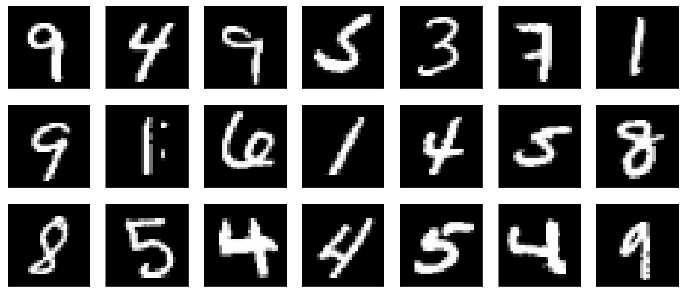
\includegraphics[width=0.9\textwidth]{images/figure8.png}
    \caption{Random sampled objects from the MNIST dataset}
    \label{fig:8}
\end{figure}

\begin{example}[MNIST]
A dataset often used as a benchmark in the context of multiclass classification is the MNIST dataset (\cite{lecun1998mnist, lecun1998gradient}), containing over $60000$ training examples $(x^{(i)}, y^{(i)}) \in \mathbb{R}^{28 \times 28} \times \{0, \ldots, 9\}$. Every object $x^{(i)}$ is a grayscale image of a handwritten digit (Figure \ref{fig:8}) and the associated label $y^{(i)}$ corresponds exactly to the respective digit. In order to use the images $x^{(i)}$ (available as matrices) as an input for a neural network, they must be vectorized (usually row-wise), such that we have an input dimension of $n_0 = 28^2 = 784$ and $n_L = 10$ as output dimension. In this example we use a neural network with depth $L=3$ and two hidden layers of width $n_1 = 100$ and $n_2 = 50$. Additionally, we apply \textcolor{blue}{\emph{batch normalization}} and \textcolor{blue}{\emph{dropout}}, techniques for a more efficient training and improving the model performance on unseen data. With a sufficient number of gradient steps optimizing the problem \ref{eqn:42}, we can determine the parameters $\hat{\boldsymbol{\theta}} = (\boldsymbol{W}^{[1]}, \boldsymbol{b}^{[1]}, \boldsymbol{W}^{[2]}, \boldsymbol{b}^{[2]}, \boldsymbol{W}^{[3]}, \boldsymbol{b}^{[3]})$, and obtain a classification accuracy of $98.37\%$ on the training data and $98.38\%$ on $10000$ unseen test images. In Figure \ref{fig:9}, we visualize a subset of rows of the matrix $\boldsymbol{W}^{[1]}$ after training and see that some rows extract certain patterns from the input data, like line segments with a certain orientation on fixed positions in the image. The activation vector $a^{[1]}$ for a fixed input $x$ thus contains information about the presence (or absence) of these geometric patterns. These information are combined in the second hidden layer to detect more complex patterns in the input, which are encoded in the activation vector $a^{[2]}$. Based on these extracted patterns, the output layer then assigns the probability of the image belonging to each class.
\end{example}

\begin{figure}[h!]
    \centering
    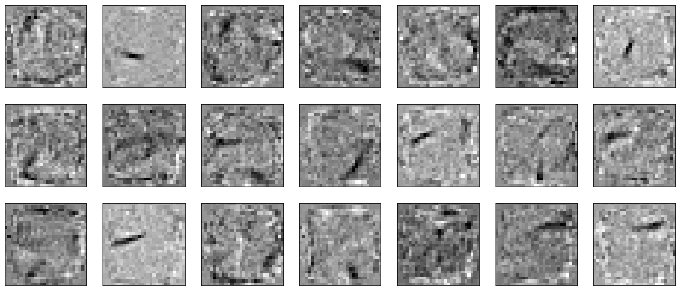
\includegraphics[width=0.9\textwidth]{images/figure9.png}
    \caption{
    Subset of rows of the weight matrix $\boldsymbol{W}^{[1]}$.The length of each row is equal to the input dimension $n_0 = 784$. Here, the rows are displayed as $28 \times 28$ grayscale images, which is the original format of the images $x^{(i)}$. Light pixels tend to correspond to positive entries, while dark pixels corresponds to negative entries and gray pixels to small absolute values.
    }
    \label{fig:9}
\end{figure}

\section{Error Backpropagation}
In order to solve the optimization problem
\begin{equation}
    \hat{\boldsymbol{\theta}} \in \argmin_{\boldsymbol{\theta} \in \Theta} \mathcal{J}(\boldsymbol{\theta}) = \argmin_{\boldsymbol{\theta} \in \Theta} \frac{1}{m} \sum_{i=1}^{m} \ell(y^{(i)}, f_\theta(x^{(i)}))
    \label{eqn:56}
\end{equation}

for a loss function $\ell$ and an artificial neural network $f_{\theta}$ with a \emph{gradient descent method}, we need to compute partial derivatives of $\ell(y^{(i)}, f_\theta(x^{(i)}))$ along the parameters $\hat{\boldsymbol{\theta}} = (\boldsymbol{W}^{[1]}, \boldsymbol{b}^{[1]}, \ldots, \boldsymbol{W}^{[L]}, \boldsymbol{b}^{[L]})$. To compute a derivative of $\mathcal{J}$ (for a fixed training data set) we simply have to sum and divide by $m$ the derivatives of $\ell(y^{(i)}, f_\theta(x^{(i)}))$. In the following, we derive the \textcolor{blue}{\emph{backpropagation}} algorithm used for this purpose (see for example \cite[section 6.5]{goodfellow2016deep}, \cite[section 5.3]{bishop2006pattern}).

\begin{figure}[h!]
    \centering
    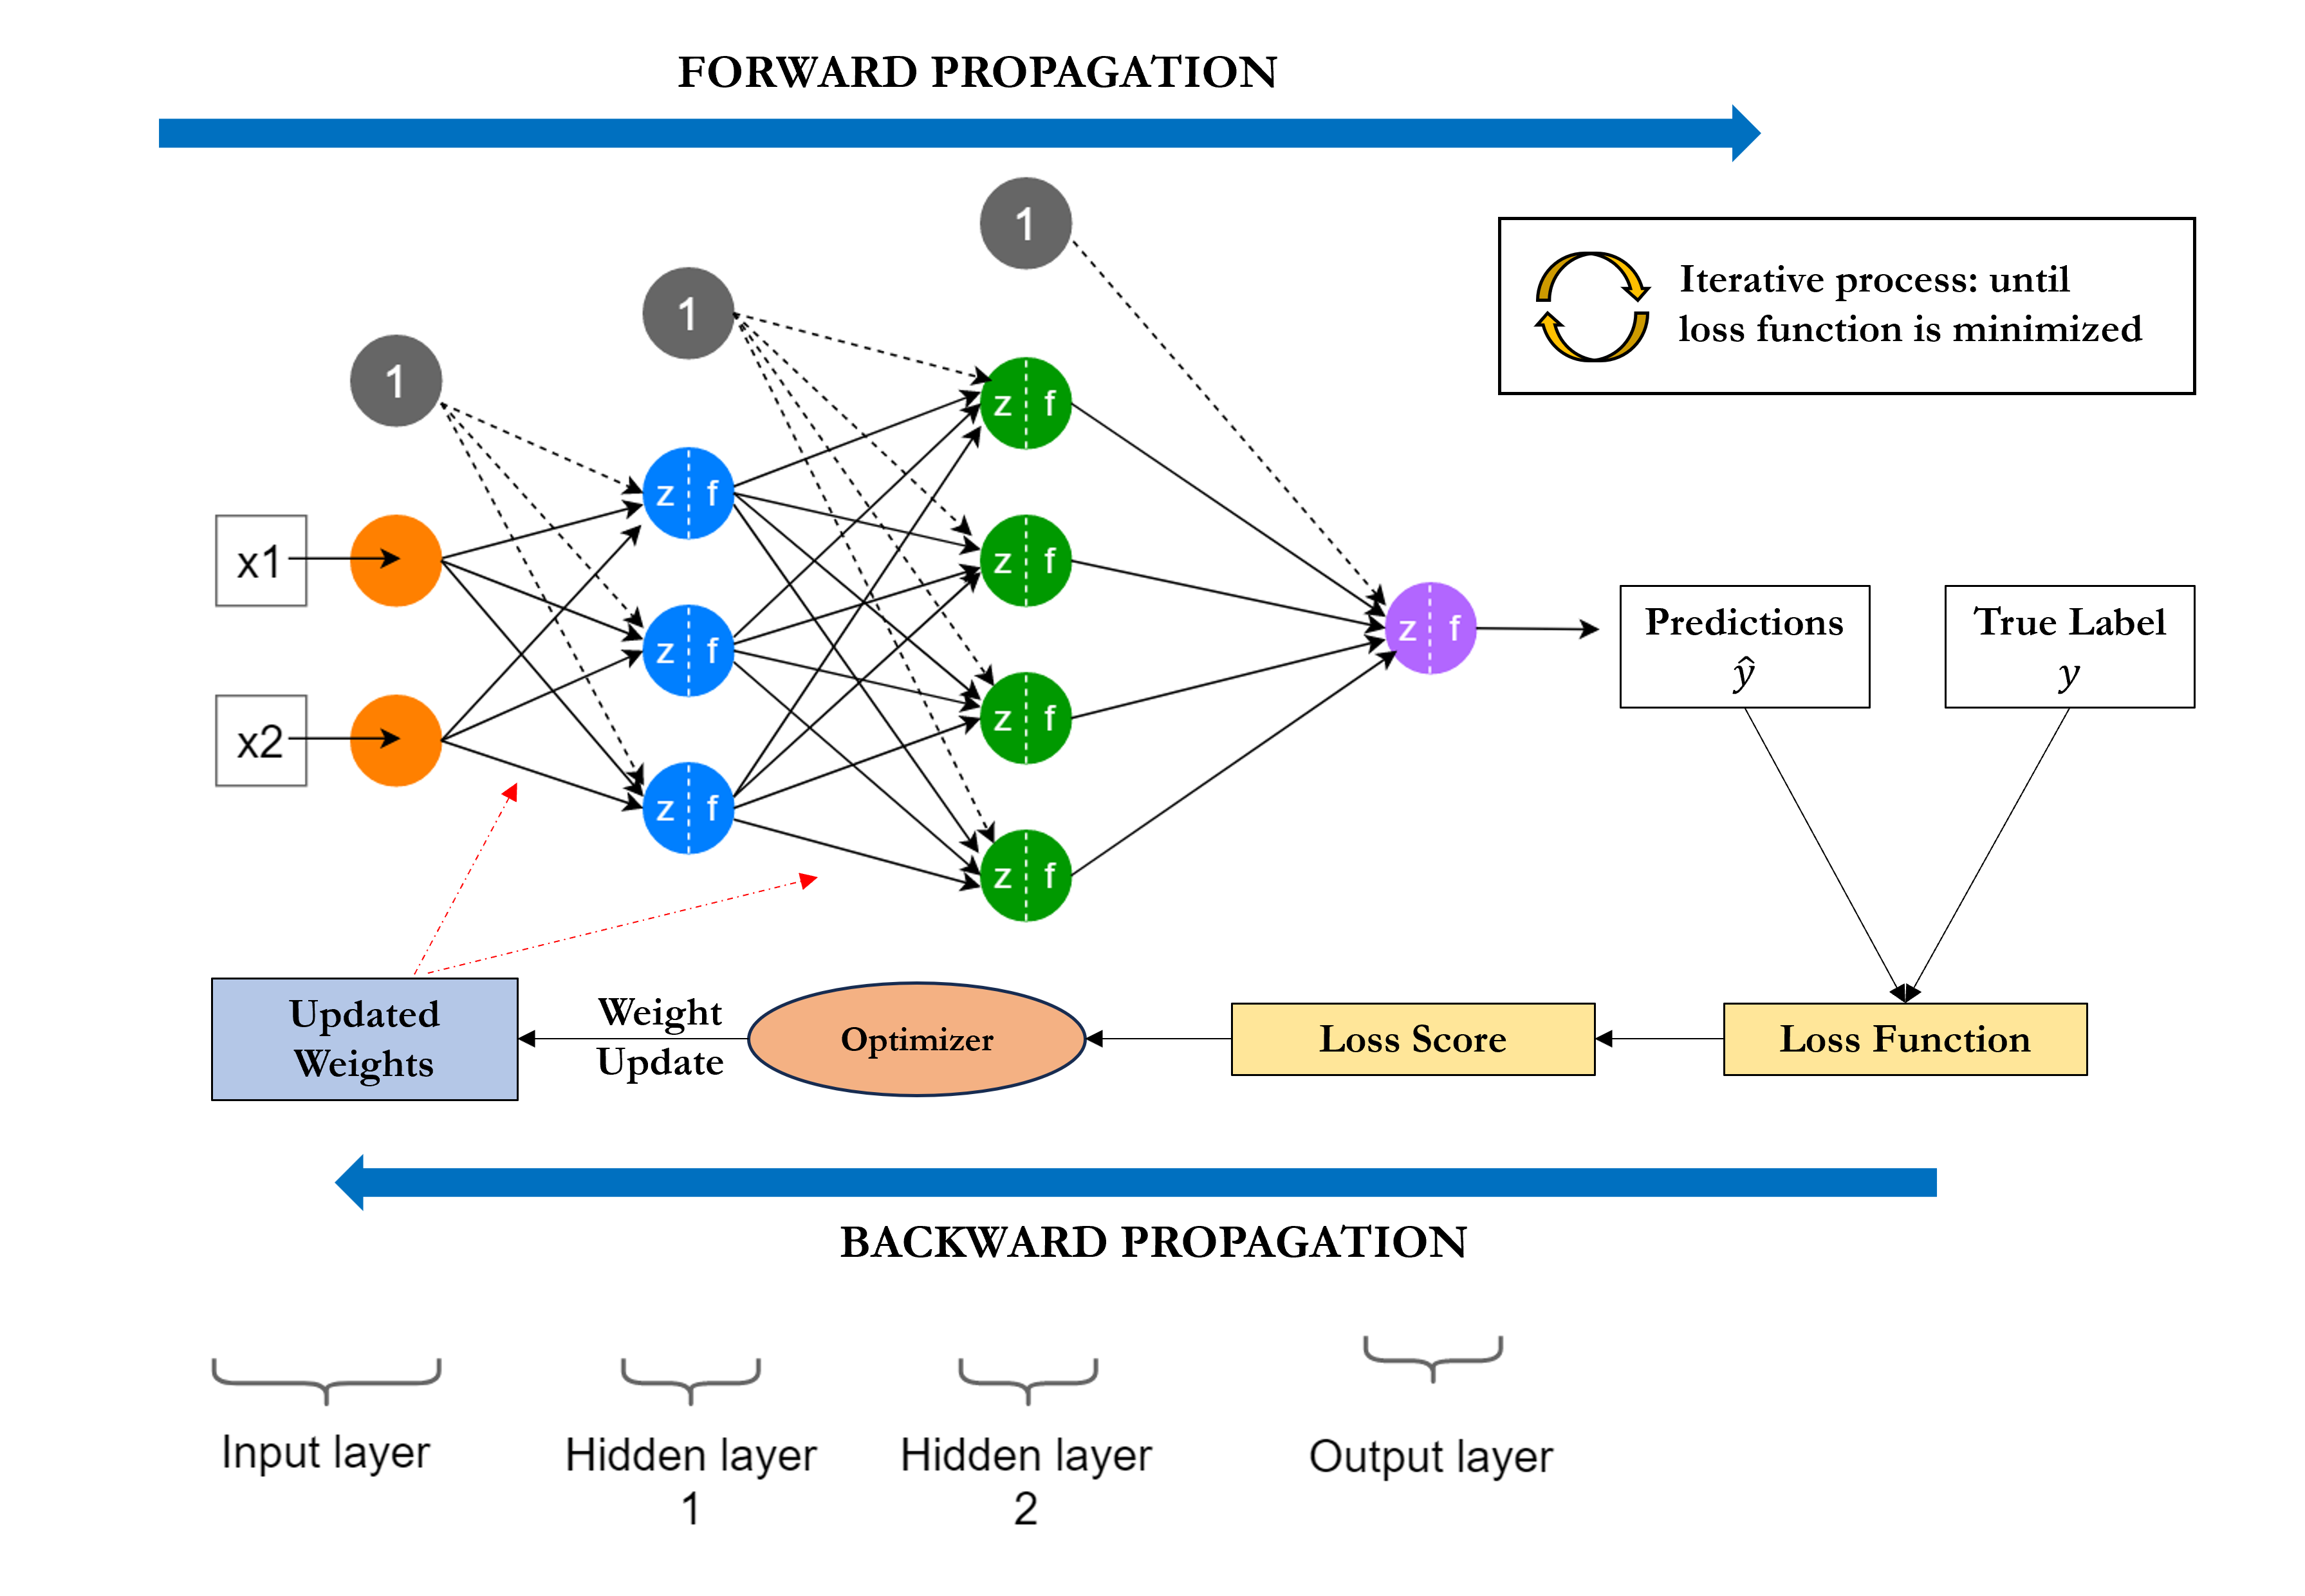
\includegraphics[width=\textwidth]{images/figure10.png}
    \caption{Illustration of how forward propagation and backward propagation works}
    \label{fig:10}
\end{figure}

\subsection{Derivatives for one Object on Parameter Basis}

\begin{lemma}[Partial derivatives with respect to parameters]\label{partial_derivative}
Let $f_{\theta}: \mathbb{R}^{n_0} \rightarrow \mathbb{R}^{n_L}$ be an artificial neural network with parameters $\hat{\boldsymbol{\theta}} = (\boldsymbol{W}^{[1]}, \boldsymbol{b}^{[1]}, \ldots, \boldsymbol{W}^{[L]}, \boldsymbol{b}^{[L]}), \ell: \mathbb{R}^{n_L} \times \mathbb{R}^{n_L} \rightarrow \mathbb{R}$, a loss function, and $(x, y) \in \mathbb{R}^{n_0} \times \mathbb{R}^{n_L}$. If we define for all $\ell \in \{1, \ldots, L\}$ and all $j \in \{1, \ldots, n_{\ell}$
\begin{equation}
    \delta_j^{[\ell]} := \frac{\partial \ell (y, f_\theta (x))}{\partial z_j^{[\ell]}} ,
    \label{eqn:57}
\end{equation}

then it holds
\begin{equation}
    \frac{\partial \ell(y, f_\theta(x))}{\partial w_{ji}^{[\ell]}} = \delta_j^{[\ell]} a_i^{[\ell-1]}
    \quad \text{and} \quad
    \frac{\partial \ell(y, f_\theta(x))}{\partial b_j^{[\ell]}} = \delta_j^{[\ell]}.
    \label{eqn:58}
\end{equation}
\end{lemma}

\textbf{\emph{Proof.}} The value of the objective function $\ell(y, f_\theta(x))$ depends exclusively on the weights $w_{ji}^{[\ell]}$ via the relation
\begin{equation}
z_j^{[\ell]} = \sum_{i=1}^{n_{\ell-1}} w_{ji}^{[\ell]} a_i^{[\ell-1]} + b_j^{[\ell]}.
\label{eqn:59}
\end{equation}

Therefore, we can apply the chain rule for the derivative and obtain
\begin{equation}
\frac{\partial \ell(y, f_\theta(x))}{\partial w_{ji}^{[\ell]}} = \frac{\partial \ell(y, f_\theta(x))}{\partial z_j^{[\ell]}} \cdot \frac{\partial z_j^{[\ell]}}{\partial w_{ji}^{[\ell]}} = \delta_j^{[\ell]} a_i^{[\ell-1]}.
\label{eqn:60}
\end{equation}

Analogously, we obtain the derivative with respect to $b_j^{[\ell]}$ with the difference that $\frac{\partial z_j^{[\ell]}}{\partial b_j^{[\ell]}} = 1$.

\begin{equation}
\frac{\partial \ell(y, f_\theta(x))}{\partial b_j^{[\ell]}} = \frac{\partial \ell(y, f_\theta(x))}{\partial z_j^{[\ell]}} \cdot \frac{\partial z_j^{[\ell]}}{\partial b_j^{[\ell]}} = \delta_j^{[\ell]}.
\label{eqn:61}
\end{equation}

Lemma \ref{partial_derivative} states that we can determine the derivatives of $\ell(y, f_{\theta}(x))$ with respect to the weights and biases with only little effort, if we know the derivatives of the respective inputs. Because partial derivatives of $\ell(y, f_\theta(x))$ depend on the derivative of the respective input vectors.

\begin{theorem}[Backpropagation]\label{backpropagation}
Let $f_{\theta}: \mathbb{R}^{n_0} \rightarrow \mathbb{R}^{n_L}$ be an artificial neural network with parameters $\hat{\boldsymbol{\theta}} = (\boldsymbol{W}^{[1]}, \boldsymbol{b}^{[1]}, \ldots, \boldsymbol{W}^{[L]}, \boldsymbol{b}^{[L]})$, loss function $\ell: \mathbb{R}^{n_L} \times \mathbb{R}^{n_L} \rightarrow \mathbb{R}$ and $(x, y) \in \mathbb{R}^{n_0} \times \mathbb{R}^{n_L}$. Furthermore, let the activation functions $g^{[1]}, \ldots, g^{[L-1]}: \mathbb{R} \rightarrow \mathbb{R}$ be defined component-wise. Then it holds for every $j \in \{1, \ldots, n_L\}$
\begin{equation}
    \delta_j^{[L]} = \sum_{k=1}^{n_L} \frac{\partial \ell(y, f_\theta(x))}{\partial a_k^{[L]}} \cdot \frac{\partial a_k^{[L]}}{\partial z_j^{[L]}}
    \label{eqn:62}
\end{equation}

and further for every $\ell \in \{1, \ldots, L-1\}$ and every $j \in \{1, \ldots, n_{\ell}\}$
\begin{equation}
    \delta_j^{[\ell]} = g^{[\ell]'}(z_j^{[\ell]}) \sum_{k=1}^{n_{\ell+1}} \delta_k^{[\ell+1]} w_{kj}^{[\ell+1]}.
    \label{eqn:63}
\end{equation}
\end{theorem}

\textbf{\emph{Proof.}} The first claim \ref{eqn:62} follows directly from the definition \ref{eqn:57} and the chain rule because the function $\ell(y, f_{\theta}(x))$ only depends on $z_j^{[L]}$ through $\boldsymbol{a}^{[L]}$. Thus
\begin{equation}
    \delta_j^{[L]} = \frac{\partial \ell(y, f_\theta(x))}{\partial z_j^{[L]}} = \underbrace{\frac{\partial \ell(y, f_\theta(x))}{\partial \boldsymbol{a}^{[L]}}}_{1 \times n_L} \cdot \underbrace{\frac{\partial \boldsymbol{a}^{[L]}}{\partial z_j^{[L]}}}_{n_L \times 1} = \sum_{k=1}^{n_L} \frac{\partial \ell(y, f_\theta(x))}{\partial a_k^{[L]}} \cdot \frac{\partial a_k^{[L]}}{\partial z_j^{[L]}}.
    \label{eqn:64}
\end{equation}

Here, $\partial \ell(y, f_\theta(x): \mathbb{R}^{n_L} \times \mathbb{R}^{n_L} \rightarrow \mathbb{R}$ and $\partial a^{[L]} \in \mathbb{R}^{n_L \times 1}$. So, the first term $\frac{\partial \ell(y, f_\theta(x))}{\partial a^{[L]}}$, which represents how the loss value (scalar) changes with respect to each component (neuron) of the activated value ($a^{[L]}$) is essentially a \textbf{Jacobian matrix} of order $1 \times n_L$.\\

Similarly, the second term, which represents how much each component (neuron) of the activated value ($\boldsymbol{a}^{[L]} \in \mathbb{R}^{n_L \times 1}$) is affected by a specific input neuron $z_j^{[L]} \in \mathbb{R}$ is a Jacobian matrix of order $n_L \times 1$.\\

By the law of matrix multiplication, the result $\delta_j^{[L]}$ is a scalar value as below:
\begin{equation}
    \begin{aligned}
    \delta_j^{[L]} &= \frac{\partial \ell(y, f_\theta(x))}{\partial z_j^{[L]}}\\
    &= \underbrace{\frac{\partial \ell(y, f_\theta(x))}{\partial \boldsymbol{a}^{[L]}}}_{1 \times n_L} \cdot \underbrace{\frac{\partial \boldsymbol{a}^{[L]}}{\partial z_j^{[L]}}}_{n_L \times 1}\\
    &= \begin{bmatrix}
        \frac{\partial \ell(y, f_\theta(x))}{\partial a_1^{[L]}} && \ldots && \frac{\partial \ell(y, f_\theta(x))}{\partial a_{n_L}^{[L]}}
    \end{bmatrix} \cdot \begin{bmatrix}
        \frac{\partial a_1^{[L]}}{\partial z_j^{[L]}} \\
        \vdots\\
        \frac{\partial a_{n_L}^{[L]}}{\partial z_j^{[L]}}
    \end{bmatrix}\\
    &= \sum_{k=1}^{n_L} \frac{\partial \ell(y, f_\theta(x))}{\partial a_k^{[L]}} \cdot \frac{\partial a_k^{[L]}}{\partial z_j^{[L]}}
    \end{aligned}
    \label{eqn:65}
\end{equation}

For the second claim, we can also apply the chain rule in a similar manner and then using the concept of matrix multiplication, express the result as a sum, as follows:
\begin{equation}
    \begin{aligned}
    \delta_{j}^{[\ell]} &= \frac{\partial \ell (y, f_{\theta} (x))}{\partial z_{j}^{[\ell]}} = \underbrace{\frac{\partial \ell (y, f_{\theta} (x))}{\partial z^{[\ell+1]}}}_{1 \times n_{\ell + 1}} \cdot \underbrace{\frac{\partial z^{[\ell+1]}}{\partial z_{j}^{[\ell]}}}_{n_{\ell + 1} \times 1}\\
    &= \sum_{k=1}^{n_{\ell+1}} \underbrace{\frac{\partial \ell (y, f_\theta (x))}{\partial z_{k}^{[\ell+1]}}}_{\delta_k^{[\ell + 1]}} \cdot \frac{\partial z_{k}^{[\ell+1]}}{\partial z_{j}^{[\ell]}} = \sum_{k=1}^{n_{\ell+1}} \delta_{k}^{[\ell+1]} \cdot \underbrace{\frac{\partial z_{k}^{[\ell+1]}}{\partial a_{j}^{[\ell]}}}_{=w_{kj}^{[\ell + 1]}} \cdot \underbrace{\frac{\partial a_{j}^{[\ell]}}{\partial z_{j}^{[\ell]}}}_{=g^{[\ell]'} \left( z_{j}^{[\ell]} \right)}\\
    &= g^{[\ell]'} \left( z_{j}^{[\ell]} \right) \sum_{k=1}^{n_{\ell+1}} \delta_{k}^{[\ell+1]} w_{kj}^{[\ell+1]}.
    \end{aligned}
    \label{eqn:66}
\end{equation}

\begin{remark}[Activation functions in the output layer]
In Theorem \ref{backpropagation}, we assumed that the activation functions $g^{[1]}, \ldots, g^{[L-1]}: \mathbb{R} \rightarrow \mathbb{R}$ are defined component-wise, while we intentionally
omitted this assumption for the activation function $g^{[L]}$ in the last layer. The reason for that is that the function $\text{softmax }: \mathbb{R}^n \rightarrow \mathbb{R}^n$ typically used as an activation in the last layer is not defined component-wise. If, in contrast, $g^{[L]}: \mathbb{R} \rightarrow \mathbb{R}$ is also defined component-wise, we obtain a simpler representation of (\ref{eqn:62}),
\begin{equation}
    \delta_j^{[L]} = \frac{\partial \ell(y, f_\theta(x))}{\partial a_j^{[L]}} \cdot \frac{\partial a_j^{[L]}}{\partial z_j^{[L]}} = g^{[L]'} \left( z_{j}^{[L]} \right) \cdot \frac{\partial \ell(y, f_\theta(x))}{\partial a_j^{[L]}}
    \label{eqn:67}
\end{equation}
\end{remark}

\begin{figure}[h!]
    \centering
    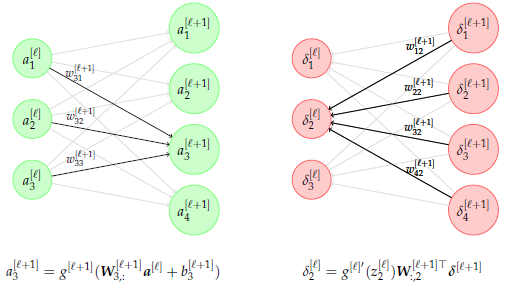
\includegraphics[width=0.8\textwidth]{images/figure11.png}
    \caption{Example for forward pass (left) vs. backpropagation (right)}
    \label{fig:11}
\end{figure}

\subsection{Vectorized Derivatives for one Object}
With Lemma \ref{partial_derivative} and Theorem \ref{backpropagation} we are now able to compute the derivatives of $\ell(y, f_\theta(x))$ with respect to $w_ji^{[\ell]}$ and $b_j^{[\ell]}$ for a fixed training example $(x, y)$. To achieve a more efficient implementation of the backpropagation it is useful to compute these derivatives \textbf{not} with respect to every single parameter but directly with respect to the whole weight matrix $\boldsymbol{W}^{[\ell]}$ and bias vector $\boldsymbol{b}^{[\ell]}$. For that, we \emph{vectorize} the derivation process.

\begin{definition}[Error]
For a fixed $(x, y) \in \mathbb{R}^{n_0} \times \mathbb{R}^{n_L}$ and $\ell \in \{1, \ldots, L\}$ we define
\begin{equation}
    \boldsymbol{\delta}^{[\ell]} := \begin{pmatrix}
        \delta_1^{[\ell]} \\ \vdots \\ \delta_{n_{\ell}}^{[\ell]}
    \end{pmatrix} \in \mathbb{R}^{n_{\ell}}
    \label{eqn:68}
\end{equation}
as the \textcolor{blue}{\emph{error}} of the $\ell$-th layer.
\end{definition}

To calculate $\boldsymbol{\delta}^{[\ell]}$, we need to distinguish the two cases $\ell = L$ and $\ell < L$, as we already did in Theorem \ref{backpropagation}. In the case $\ell = L$ we can directly expand the definition to

\begin{equation}
    \begin{aligned}
    \boldsymbol{\delta}^{[L]\top} &= \frac{\partial \ell(y, f_\theta(x))}{\partial \boldsymbol{z}^{[L]}} = \frac{\partial \ell(y, f_\theta(x))}{\partial \boldsymbol{a}^{[L]}} \cdot \frac{\partial \boldsymbol{a}^{[L]}}{\partial \boldsymbol{z}^{[L]}}\\
    &= \underbrace{\begin{pmatrix}
        \frac{\partial \ell(y, f_\theta(x))}{\partial a_1^{[L]}} \cdots \frac{\partial \ell(y, f_\theta(x))}{\partial a_{n_L}^{[L]}}
    \end{pmatrix}}_{1 \times n_L} \underbrace{\begin{pmatrix}
        \frac{\partial a_1^{[L]}}{\partial z_1^{[L]}} & \cdots & \frac{\partial a_1^{[L]}}{\partial z_{n_L}^{[L]}}\\
        \vdots & \ddots & \vdots\\
        \frac{\partial a_{n_L}^{[L]}}{\partial z_1^{[L]}} & \cdots & \frac{\partial a_{n_L}^{[L]}}{\partial z_{n_L}^{[L]}}
    \end{pmatrix}}_{n_L \times n_L}
    \end{aligned}
    \label{eqn:69}
\end{equation}

By analogy with (\ref{eqn:67}) we obtain,
\begin{equation}
    \boldsymbol{\delta}^{[L]} = g^{[L]'} \left( \boldsymbol{z}^{[L]} \right) \odot \left[ \frac{\partial \ell (y, f_\theta(x))}{\partial \boldsymbol{a}^{[L]}}  \right]^\top = g^{[L]'} \left( \boldsymbol{z}^{[L]} \right) \odot \nabla_{\boldsymbol{a}^{[L]}} \ell(y, f_\theta(x))
    \label{eqn:70}
\end{equation}

for a component-wise defined $g^{[L]}: \mathbb{R} \rightarrow \mathbb{R}$, where $g^{[L]'}: \mathbb{R} \rightarrow \mathbb{R}$ is also applied component-wise to $z^{[L]}$. Here, with $\odot$ we denote the component-wise multiplication of two vectors. Note that in this case $\partial \boldsymbol{a}^{[L]} / \partial \boldsymbol{z}^{[L]}$ is a diagonal matrix with entries $g^{[L]'} \left( z_j^{[L]} \right), j= 1, \ldots, n_L$.

\begin{remark}
In several cases of interest (e.g., when $g^{[L]}$ is the softmax function (\ref{eqn:38})) it holds
\begin{equation}
    \boldsymbol{\delta}^{[L]} = \boldsymbol{f_\theta(x)} - \boldsymbol{y}
    \label{eqn:71}
\end{equation}
\end{remark}

\textbf{\emph{Proof.}} From \ref{eqn:41}, we can see the softmax loss function as:
\begin{equation}
    \ell(y, f_\theta(x)) = - \sum_{k=1}^{K}y_k \ln(f_\theta(x)_k)
    \label{eqn:72}
\end{equation}
where,
$K = n_L$ is the number of categories or neurons in the final layer, $y_k \in \{0,1\}$ is the true label of the $k$-th category. If $y_k = a_k^{[L]} = 1$ (true), then all other $y_j a_j^{[L]} = 0$ for $j \neq k$. Also, $\sum_{k=1}^{K}y_k =1$ holds. $f_\theta(x)_k$ is the output of the neural network, which gives us the probability of the $k$-th category.\\

From \ref{eqn:62}, it follows:
\begin{equation}
    \begin{aligned}
    \delta_j^{[L]} &= \frac{\partial \ell(y, f_\theta(x))}{\partial z_j^{[L]}} = \sum_{k=1}^{n_L} \frac{\partial \ell(y, f_\theta(x))}{\partial a_k^{[L]}} \cdot \frac{\partial a_k^{[L]}}{\partial z_j^{[L]}}\\
    &= \sum_{k=1}^{n_L} \left[ \frac{\partial}{\partial a_k^{[L]}} \left(- \sum_{n=1}^{n_L}y_n \ln(f_\theta(x)_n)\right) \cdot \frac{\partial}{\partial z_j^{[L]}} \left( a_k^{[L]} \right) \right]\\
    & = \sum_{k=1}^{n_L} \left[ \left(- \sum_{n=1}^{n_L}y_n \frac{\partial \ln(f_\theta(x)_n)}{\partial a_k^{[L]}} \right) \cdot \frac{\partial}{\partial z_j^{[L]}} \left( \frac{e^{z_k}}{\sum_{i=1}^{n_L}e^{z_i}} \right) \right]\\
    \end{aligned}
    \label{eqn:73}
\end{equation}

Using the formula $\frac{\partial}{\partial x}\left( \frac{f(x)}{g(x)} \right) = \frac{f'(x)g(x) - f(x)g'(x)}{g(x)^2}$ for the second part of the above equation, we get:

\begin{equation}
    = \sum_{k=1}^{n_L} \left[ \left(- \sum_{n=1}^{n_L}y_n \frac{\partial \ln(f_\theta(x)_n)}{\partial a_k^{[L]}} \right) \cdot (\delta_{k,j}f_\theta(x)_k - f_\theta(x)_k f_\theta(x)_j) \right]\\
    \label{eqn:74}
\end{equation}

where $\delta_{k,j}$ is the \textcolor{blue}{\emph{Kronecker delta}}, which is equal to $1$ if $k=j$ and $0$ otherwise.\\

Proceeding further using the concept that $f_\theta(x)_k = a_k^{[L]}$ for the first part, we get:
\begin{equation}
    \begin{aligned}
    &= \sum_{k=1}^{n_L} \left[ - \frac{y_k}{f_\theta(x)_k} (\delta_{k,j}f_\theta(x)_k - f_\theta(x)_k f_\theta(x)_j) \right] \quad \text{(First term: only $n=k$ survives)}\\
    &= \sum_{k=1}^{n_L} \left[ y_k f_\theta(x)_j - \delta_{k,j} y_k  \right]\\
    &= \sum_{k=1}^{n_L} y_k f_\theta(x)_j - \sum_{k=1}^{n_L} \delta_{k,j} y_k\\
    &= f_\theta(x)_j \sum_{k=1}^{n_L} (y_k) - y_j \quad \text{(Since, $\delta_{k,j} = 1$ only for $k=j$ and $0$ otherwise)}\\
    &= f_\theta(x)_j -y_j \quad \text{(Since, $\sum_{k=1}^{n_L} y_k = 1$)}\\
    \end{aligned}
    \label{eqn:75}
\end{equation}

Finally, we get:
\begin{equation}
    \delta_j^{[L]} = f_\theta(x)_j - y_j
    \label{eqn:76}
\end{equation}

From that, it immediately follows:
\begin{equation}
    \boldsymbol{\delta}^{[L]} = \boldsymbol{f_\theta(x)} - \boldsymbol{y},
    \label{eqn:77}
\end{equation}
when the activation function in the final layer i.e., $g^{[L]}$ is the \emph{softmax function}.\\

Now consider the second case $\ell < L$. With (\ref{eqn:63}) we can directly see that
\begin{equation}
    \delta_j^{[\ell]} = g^{[\ell]'}(z_j^{[\ell]}) \sum_{k=1}^{n_{\ell+1}} \delta_k^{[\ell+1]} w_{kj}^{[\ell+1]} = g^{[\ell]'}(z_j^{[\ell]}) \boldsymbol{W}_{:,j}^{[\ell +1]\top} \boldsymbol{\delta}^{[\ell +1]}
    \label{eqn:78}
\end{equation}

holds where by $\boldsymbol{W}_{:,j}^{[\ell +1]}$, we denote the $j$-th column of the weight matrix of the $(\ell +1)$-th layer (see example in Figure \ref{fig:11}). With that, it follows:

\begin{equation}
    \boxed{
    \delta^{[\ell]} = g^{[\ell]}(z^{[\ell]}) \odot \boldsymbol{W}^{[\ell+1]^\top} \boldsymbol{\delta}^{[\ell+1]} }
    \label{eqn:79}
\end{equation}

Finally we also want to use the error $\boldsymbol{\delta}^{[\ell]}$ to obtain the derivatives with respect to the weights $\boldsymbol{W}^{[\ell]}$ and biases $\boldsymbol{b}^{[\ell]}$ in a vectorized form. Based on (\ref{eqn:58}), we obtain:
\begin{equation}
    \begin{aligned}
    &\frac{\partial \ell(y, f_\theta(x))}{\partial w_{ji}^{[\ell]}} = \delta_j^{[\ell]} a_i^{[\ell-1]}\\
    \Rightarrow &\nabla_{\boldsymbol{W}_{j,:}^{[\ell]}} \ell(y, f_\theta(x)) = \delta_j^{[\ell]} \boldsymbol{a}^{[\ell-1]^\top}\\
    \Rightarrow &\boxed{\nabla_{\boldsymbol{W}^{[\ell]}} \ell(y, f_\theta(x)) = \boldsymbol{\delta}^{[\ell]} \boldsymbol{a}^{[\ell-1]^\top}}
    \end{aligned}
    \label{eqn:80}
\end{equation}

and
\begin{equation}
    \begin{aligned}
    &\frac{\partial \ell(y, f_\theta(x))}{\partial b_j^{[\ell]}} = \delta_j^{[\ell]} \\
    \Rightarrow &\boxed{\nabla_{\boldsymbol{b}^{[\ell]}} \ell(y, f_\theta(x)) = \boldsymbol{\delta}^{[\ell]}}
    \end{aligned}
    \label{eqn:81}
\end{equation}

\begin{algorithm}
\caption{(Vectorized Backpropagation for one Training Object)}
\textbf{Input:} $x, y, g^{[1]}, \dots, g^{[L]}, \theta = (W^{[1]}, b^{[1]}, \dots, W^{[L]}, b^{[L]})$ \\
\textbf{Output:} $\nabla_\theta \ell(y, f_\theta(x))$\\

\begin{algorithmic}[1]
\STATE $a^{[0]} := x$ \hfill $\triangleright$ Forward pass
\FOR{$\ell = 1, \dots, L$}
    \STATE $z^{[\ell]} := W^{[\ell]} a^{[\ell-1]} + b^{[\ell]}$
    \STATE $a^{[\ell]} := g^{[\ell]}(z^{[\ell]})$
\ENDFOR
\STATE
\STATE $\delta^{[L]} = \nabla_{z^{[L]}} \ell(y, f_\theta(x))$ \hfill $\triangleright$ Error backpropagation
\FOR{$\ell = L, \dots, 1$}
    \STATE $\delta^{[\ell]} := g^{[\ell]'}(z^{[\ell]}) \odot W^{[\ell+1]\top} \delta^{[\ell+1]}$
    \STATE $\nabla_{W^{[\ell]}} := \delta^{[\ell]} a^{[\ell-1]\top}$
    \STATE $\nabla_{b^{[\ell]}} := \delta^{[\ell]}$
\ENDFOR
\STATE
\STATE \textbf{return} $\nabla_\theta \ell(y, f_\theta(x)) = (\nabla_{W^{[1]}}, \nabla_{b^{[1]}}, \dots, \nabla_{W^{[L]}}, \nabla_{b^{[L]}})$
\end{algorithmic}
\end{algorithm}


\vspace{5em}
\textbf{TO BE CONTINUED...}


